\documentclass[xetex,mathserif,serif]{beamer}
\usepackage{polyglossia}
\setdefaultlanguage[babelshorthands=true]{russian}
\usepackage{minted}
\usepackage{tabu}

\useoutertheme{infolines}

\usepackage{fontspec}
\setmainfont{FreeSans}
\newfontfamily{\russianfonttt}{FreeSans}

\tabulinesep=0.7mm

\title{Лекция 9: Антипаттерны}
\subtitle{То, как делать не надо}
\author[Юрий Литвинов]{Юрий Литвинов \newline \textcolor{gray}{\small\texttt{yurii.litvinov@gmail.com}}}

\date{08.11.2019г}

\begin{document}
	
	\frame{\titlepage}

	\section{Введение}

	\begin{frame}
		\frametitle{Антипаттерны --- что это и зачем?}
		\begin{itemize}
			\item Часто встречающиеся решения, приводящие к известным проблемам
			\begin{itemize}
				\item Сами по себе решения могут быть неплохи, может быть плох контекст их применения
			\end{itemize}
			\item Так же, как и паттерны, нужны для введения общего словаря и общеизвестного набора решений
			\item Описание антипаттерна должно содержать не только проблему, но и то, почему это решение плохо, и как сделать хорошо
			\item Бывают разные виды, относящиеся к разным сферам деятельности
			\begin{itemize}
				\item Антипаттерны реализации
				\begin{itemize}
					\item В том числе, специфичные для конкретного языка или технологии
				\end{itemize}
				\item Архитектурные антипаттерны
				\item Антипаттерны организации
			\end{itemize}
		\end{itemize}
	\end{frame}

	\begin{frame}
		\frametitle{Книжка}
		\begin{columns}
			\begin{column}{0.6\textwidth}
				AntiPatterns: Refactoring Software, Architectures, and Projects in Crisis by William J. Brown, Raphael C. Malveau, SkipMcCormick, Thomas J. Mowbray, Wiley, 1998, 336pp.
			\end{column}
			\begin{column}{0.4\textwidth}
				\begin{center}
					
\includegraphics[width=\textwidth]{bookCover.png}
				\end{center}
			\end{column}
		\end{columns}
	\end{frame}

	\begin{frame}
		\frametitle{Семь причин провала проектов}
		\begin{footnotesize}
			\begin{itemize}
				\item Спешка
				\begin{itemize}
					\item Look you --- just ``clean up'' the code. We ship tomorrow.
				\end{itemize}
				\item Апатия --- неприменение известных хороших решений
				\begin{itemize}
					\item Reuse? Who’s ever gonna reuse this crappy code? NO ONE! That’s who.
				\end{itemize}
				\item Недалёкость --- незнание хороших решений
				\begin{itemize}
					\item I don’t need to know and I don’t care to know.
				\end{itemize}
				\item Лень --- следование пути наименьшего сопротивления
				\item Архитектурная жадность --- излишняя детальность
				\begin{itemize}
					\item Well, it certainly is complicated! I’m sure our clients will be very, very impressed.
				\end{itemize}
				\item Неведение --- нежелание понимать
				\item Гордость --- нежелание переиспользовать готовые решения
				\begin{itemize}
					\item Not-invented-here syndrome.
				\end{itemize}
			\end{itemize}
		\end{footnotesize}
	\end{frame}

	\section{Антипаттерны реализации}

	\begin{frame}
		\frametitle{Circular dependency}
		\begin{itemize}
			\item Два или больше компонентов, которые зависят друг от друга
			\begin{itemize}
				\item Зависимости модулей должны образовывать ациклический граф
			\end{itemize}
			\item Часто появляется как результат попыток добавить callback-и
			\begin{itemize}
				\item Или просто по неосторожности
			\end{itemize}
			\item Имеет впечатляющие последствия в C++, во многих языках невозможен
			\item Как бороться:
			\begin{itemize}
				\item Зависеть от абстракции, а не от реализации
				\item Разделение на слои
				\item Observer, Dependency Injection и т.д.
			\end{itemize}
		\end{itemize}
	\end{frame}

	\begin{frame}
		\frametitle{Sequential coupling}
		\begin{itemize}
			\item Необходимость вызывать методы класса в определённом порядке
			\begin{itemize}
				\item Например, вызов init() после конструктора
				\item Бывают более запущенные случаи, когда есть целая цепочка методов
			\end{itemize}
			\item Как бороться:
			\begin{itemize}
				\item Шаблонный метод
				\item Фабрики и строители
			\end{itemize}
		\end{itemize}
	\end{frame}

	\begin{frame}
		\frametitle{Call super}
		\begin{itemize}
			\item Необходимость вызывать из переопределённого метода потомка переопределяемый метод предка
			\begin{itemize}
				\item Не может быть проверено компилятором
			\end{itemize}
			\item Как бороться:
			\begin{itemize}
				\item Template Method
				\begin{itemize}
					\item \textbf{Позволяет} переопределить поведение предка, а не \textbf{требует} этого
				\end{itemize}
			\end{itemize}
		\end{itemize}
	\end{frame}

	\begin{frame}
		\frametitle{Yo-yo problem}
		\begin{itemize}
			\item Развитие идеи Call Super --- а давайте предок будет тоже вызывать виртуальные методы, переопределённые в потомке, которые будут вызывать методы предка и т.д.
			\begin{itemize}
				\item Красивая объектно-ориентированная архитектура же!
			\end{itemize}
			\item Как бороться:
			\begin{itemize}
				\item Перераспределить функциональность между предками и потомками
				\item Возможно, распилить иерархию на несколько
				\begin{itemize}
					\item Паттерн ``Мост''
				\end{itemize}
				\item Вообще избегать глубоких иерархий наследования
				\begin{itemize}
					\item И ещё более вообще, использовать наследование только для полиморфных вызовов
				\end{itemize}
			\end{itemize}
		\end{itemize}
	\end{frame}

	\begin{frame}
		\frametitle{Busy waiting}
		\begin{itemize}
			\item Ожидание наступления некоторого события в бесконечном цикле с неблокирующими вызовами проверки наступления события
			\begin{itemize}
				\item Ещё использование циклов для задержек
			\end{itemize}
			\item Не всегда плохо, может быть валидным решением на встроенных устройствах
			\begin{itemize}
				\item И на самом деле используется в реализации примитивов синхронизации типа мониторов
			\end{itemize}
			\item Как бороться:
			\begin{itemize}
				\item Использовать планировщик: блокирующие вызовы, ``усыпляющие'' поток до наступления события
				\begin{itemize}
					\item select в linux
					\item Мьютексы, condition\_variable и т.д.
				\end{itemize}
				\item Использовать аппаратные возможности: таймеры и прерывания
			\end{itemize}
		\end{itemize}
	\end{frame}

	\begin{frame}
		\frametitle{Error hiding}
		\begin{itemize}
			\item Сообщение об ошибке прячется за ``дружественным к пользователю'' сообщением или прячется вообще
			\begin{itemize}
				\item В худшем случае информация об ошибке теряется окончательно
			\end{itemize}
			\item Как бороться:
			\begin{itemize}
				\item Давать программе упасть (ещё, принцип ``fail fast'')
				\item Логировать все исключения
			\end{itemize}
		\end{itemize}
	\end{frame}

	\begin{frame}
		\frametitle{Magic numbers, Magic strings}
		\begin{itemize}
			\item Внезапно появляющиеся в коде программы строковые или числовые литералы
			\begin{itemize}
				\item 0, 1 и т.д. не считаются
			\end{itemize}
			\item Особенно забавно, если автор любезно посчитал значение математического выражения и записал в код результат
			\item Как бороться:
			\begin{itemize}
				\item Константы
				\item Ресурсы для локализации
			\end{itemize}
		\end{itemize}
	\end{frame}

	\section{Антипаттерны проектирования}

	\begin{frame}
		\frametitle{God Object (The Blob)}
		``This is the class that is really the heart of our architecture.''
		\begin{itemize}
			\item Один класс управляет всем процессом вычислений, остальные в основном предоставляют ему данные
			\begin{itemize}
				\item Привычка к структурному программированию, разделение данных и кода
				\item Постепенная эволюция proof-of-concept без рефакторинга (лень, спешка)
				\item Архитектурная ошибка, неправильное разделение обязанностей
			\end{itemize}
			\item Хаотичное объединение различных ответственностей в один класс
			\begin{itemize}
				\item Больше 60 полей и методов могут указывать на God Object
				\begin{itemize}
					\item При этом String вряд ли так можно классифицировать
				\end{itemize}
			\end{itemize}
			\item Исключения: обёртки над legacy-компонентами
			\begin{itemize}
				\item Их нет нужды декомпозировать
			\end{itemize}
		\end{itemize}
	\end{frame}

	\begin{frame}
		\frametitle{God Object, что делать}
		\begin{itemize}
			\item Передать больше ответственности классам-данным
			\item Разделить методы класса на группы, соответствующие контрактам, выполняемым God Object-ом
			\item Поискать среди уже существующих классов более подходящие для каждой группы методов
			\item При необходимости создать новые классы, в соответствии с принципом единственности ответственности
			\item Убрать непрямые зависимости (если объекты A и B лежат внутри объекта G, может так случиться, что A может быть в B, а B --- в G)
		\end{itemize}
	\end{frame}

	\begin{frame}
		\frametitle{Swiss Army Knife}
		\begin{itemize}
			\item Swiss Army Knife --- класс с чрезмерно сложным интерфейсом, который пытается уметь делать всё, что в принципе может понадобиться
			\begin{itemize}
				\item Часто появляется в библиотеках как результат попыток вендора сделать свою технологию возможно более применимой
			\end{itemize}
			\item Инкапсуляция сложности приносится в жертву гибкости, что лишает абстракцию смысла
			\item Отличается от God Object-а тем, что не пытается монополизировать управление
			\begin{itemize}
				\item Швейцарских ножей может быть много
				\item God Object часто имеет очень простой public-интерфейс
			\end{itemize}
		\end{itemize}
	\end{frame}

	\begin{frame}
		\frametitle{Lava Flow}
		\begin{footnotesize}
			``Oh that! Well Ray and Emil (they’re no longer with the company) wrote that routine back when Jim (who left last month) was trying a workaround for Irene’s input processing code (she’s in another department now, too). I don’t think it’s used anywhere now, but I’m not really sure. Irene didn’t really document it very clearly, so we figured we would just leave well enough alone for now. After all, the bloomin’ thing works doesn’t it?!''
		\end{footnotesize}
		\vspace{0.3cm}
		\begin{itemize}
			\item Мёртвый код и незакрытый технический долг ``застывают'' в системе, как потоки лавы
			\begin{itemize}
				\item Появляется он, как правило, как эксперименты, ``костыли'' или быстрые фиксы
				\item Люди, писавшие их, уходят из команды, оставшиеся не имеют идей, что это, но трогать боятся (спешка, лень)
				\begin{itemize}
					\item ``It doesn’t really cause any harm, and might actually be critical, and we just don’t have time to mess with it.''
				\end{itemize}
			\end{itemize}
			\item Закомментированный код, куча TODO, большие методы без комментариев, непонятные интерфейсы
		\end{itemize}
	\end{frame}

	\begin{frame}
		\frametitle{Lava Flow, что делать}
		\begin{itemize}
			\item Как предупредить:
			\begin{itemize}
				\item Не писать production-код до продумывания архитектуры
				\item Активно использовать контроль версий с ветками
			\end{itemize}
			\item Как лечить:
			\begin{itemize}
				\item Остановить разработку и провести архитектурный реинжиниринг
				\begin{itemize}
					\item Сложный и долгий процесс анализа существующей системы и создания to-be-архитектуры
				\end{itemize}
				\item Постепенное вырезание мёртвого кода приведёт к багам, их нельзя фиксить новыми костылями
				\item Выкинуть и написать заново?
			\end{itemize}
		\end{itemize}
	\end{frame}

	\begin{frame}
		\frametitle{Functional Decomposition}
		``This is our ‘main’ routine, here in the class called LISTENER.''
		\begin{itemize}
			\item Программирование путём разделения задачи на вызывающие друг друга функции
			\begin{itemize}
				\item Не анти-паттерн для структурного программирования (Pascal, Ada, C) и, тем более, функционального программирования (хотя тут возможны варианты)
				\begin{itemize}
					\item Высокоуровневая декомпозиция модулей системы по функциям тоже ок
				\end{itemize}
			\end{itemize}
			\item Классы с ``функциональными'' именами, классы с одним методом, классы с кучей private-методов
		\end{itemize}
	\end{frame}

	\begin{frame}
		\frametitle{Functional Decomposition, что делать}
		\begin{itemize}
			\item Вернуться к требованиям, построить модель предметной области
			\item Отобразить требования и модель на существующий код
			\begin{itemize}
				\item Цель --- объяснить и задокументировать то, что уже написано
			\end{itemize}
			\item Классы с одним методом прибить, переместив их код в другие классы
			\begin{itemize}
				\item Хелперы, например
			\end{itemize}
			\item Собрать несколько классов в один, который бы отвечал за что-то разумное из предметной области или требований
			\item Если в классе нет состояния, имеет смысл сделать его функцией или статическим классом
			\begin{itemize}
				\item Состояние имеет свойство заводиться само по мере рефакторинга
			\end{itemize}
			\item Сделать из основного метода God Object, а дальше понятно, что делать
		\end{itemize}
	\end{frame}

	\begin{frame}
		\frametitle{Poltergeists}
		``I’m not exactly sure what this class does, but it sure is important!''
		\begin{itemize}
			\item Классы, которые не нужны архитектуре системы и существуют лишь чтобы выполнить какие-то действия с другими классами
			\begin{itemize}
				\item ...Controller, ...Manager и т.д., нужные только для инициализации или вызова других классов
				\item Время жизни их объектов ограничено (отсюда название)
				\item Тенденция использовать побочные эффекты
				\begin{itemize}
					\item Вся идиома RAII в C++
				\end{itemize}
			\end{itemize}
		\end{itemize}
	\end{frame}

	\begin{frame}
		\frametitle{Golden Hammer}
		``I have a hammer and everything else is a nail.'', ``Our database is our architecture.'', ``Maybe we shouldn’t have used Excel macros for this job after all.''
		\begin{itemize}
			\item Рост опыта во владении конкретным продуктом, технологией или стеком пропорционален желанию использовать их везде, где только можно
			\begin{itemize}
				\item Усугубляется желанием вендоров выпускать кучу расширений
				\item Иногда это осмысленно, чаще нет
				\begin{itemize}
					\item Пересесть на новый язык программирования и стек технологий занимает не больше недели!
				\end{itemize}
				\item Собственно, антипаттерн --- даже не хотеть погуглить
			\end{itemize}
			\item Создаваемые решения испытывают сильное влияние конкретной технологии, используемой для их разработки
			\item Большие вложения в молоток, которые жалко терять
		\end{itemize}
	\end{frame}

	\begin{frame}
		\frametitle{Golden Hammer, как бороться}
		\begin{itemize}
			\item Психологические аспекты, которых мы здесь не касаемся
			\item Обучение
			\begin{itemize}
				\item Внутрикорпоративные семинары
				\item Поездки на конференции
			\end{itemize}
			\item Разделение системы на заменяемые компоненты
			\begin{itemize}
				\item Сервисно-ориентированная (микросервисная) архитектура
				\item Следование индустриальным стандартам при определении границ компонентов
				\item Использование ``кросс-технологических'' инструментов (Protobuf, Thrift, ...)
			\end{itemize}
			\item Не бояться нового
			\begin{itemize}
				\item Квалифицированный программист может хорошо программировать на чём угодно
			\end{itemize}
		\end{itemize}
	\end{frame}

	\section{Design smells}

	\begin{frame}
		\frametitle{Design smells}
		\begin{itemize}
			\item \textbf{Missing abstraction} --- использование примитивных или слишком общих типов данных вместо своих классов
			\item \textbf{Multifaceted abstraction} --- нарушение единственности ответственности
			\item \textbf{Duplicate abstraction} --- две абстракции имеют одно предназначение
			\item \textbf{Deficient encapsulation} --- слишком широкая видимость
			\item \textbf{Unexploited encapsulation} --- явные проверки типов вместо полиморфизма
		\end{itemize}
	\end{frame}

	\begin{frame}
		\frametitle{Design smells (2)}
		\begin{itemize}
			\item \textbf{Broken modularization} --- неуместное разбиение на классы/пакеты
			\item \textbf{Insufficient modularization} --- неуместное неразбиение на классы/пакеты
			\item \textbf{Cyclically-dependent modularization} --- циклические зависимости
			\item \textbf{Unfactored hierarchy} --- дупликация в иерархии
			\item \textbf{Broken hierarchy} --- нарушение принципа подстановки и IS-A
			\item \textbf{Cyclic hierarchy} --- зависимость от потомков
		\end{itemize}
	\end{frame}

	\section{Антипаттерны архитектуры}

	\begin{frame}
		\frametitle{Stovepipe Enterprise (Island of Automation)}
		\begin{columns}
			\begin{column}{0.6\textwidth}
				\begin{itemize}
					\item Отсутствие переиспользования между системами в организации или между компонентами в одной системе
					\begin{itemize}
						\item Существующие кодовые базы никак не помогают друг другу
					\end{itemize}
					\item Как бороться:
					\begin{itemize}
						\item Использовать промышленные стандарты
						\item Фиксировать технологии и типовую архитектуру на уровне предприятия
						\item Создать и поддерживать инфраструктуру переиспользования
					\end{itemize}
				\end{itemize}
			\end{column}
			\begin{column}{0.4\textwidth}
				\begin{center}
					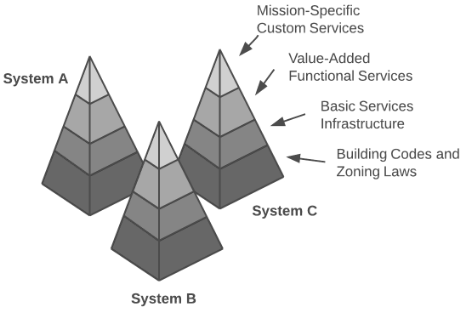
\includegraphics[width=\textwidth]{islandOfAutomation.png} \\
					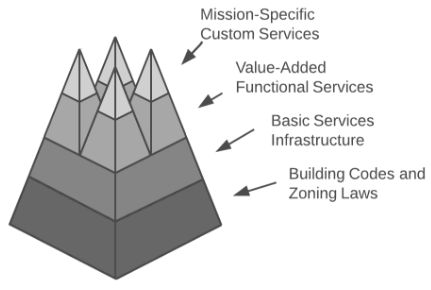
\includegraphics[width=\textwidth]{noIslandOfAutomation.png}
				\end{center}	
			\end{column}
		\end{columns}
	\end{frame}

	\begin{frame}
		\frametitle{Stovepipe System}
		\begin{columns}
			\begin{column}{0.7\textwidth}
				\begin{itemize}
					\item Аналог Stovepipe Enterprise для отдельной системы
					\begin{itemize}
						\item Отсутствие единого стандарта по взаимодействию между подсистемами
						\item Интеграция между подсистемами по принципу ad-hoc
					\end{itemize}
					\item Как бороться:
					\begin{itemize}
						\item Абстракция --- единые интерфейсы для подсистем
						\item Единый протокол общения между подсистемами
						\begin{itemize}
							\item Паттерны интеграции, например, Enterprise Service Bus
						\end{itemize}
					\end{itemize}
				\end{itemize}
			\end{column}
			\begin{column}{0.3\textwidth}
				\begin{center}
					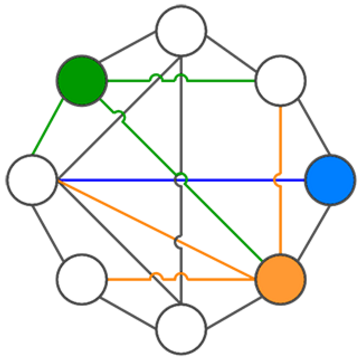
\includegraphics[width=\textwidth]{stovepipeSystem.png}
				\end{center}	
			\end{column}
		\end{columns}
	\end{frame}

	\begin{frame}
		\frametitle{Vendor Lock−In}
		\begin{itemize}
			\item Жёсткая зависимость архитектуры или реализации от третьестороннего коммерческого решения
			\item Приложения могут жить очень долго и легко переживают вендоров третьесторонних компонент или инструментов
			\item Как бороться:
			\begin{itemize}
				\item Программировать не ``на'', а ``с помощью''
				\item Изоляционный слой
				\item Реинжиниринг
			\end{itemize}
		\end{itemize}
	\end{frame}

	\begin{frame}
		\frametitle{Architecture By Implication}
		\begin{itemize}
			\item Отсутствие явных архитектурных спецификаций для разрабатываемой системы
			\begin{itemize}
				\item ``We’ve done systems like this before!'', ``There is no risk; we know what we’re doing!''
			\end{itemize}
			\item Скрытые риски, возможное недопонимание, ``Золотой молоток''
			\item Как бороться:
			\begin{itemize}
				\item Фиксировать формат описания архитектуры системы
				\begin{itemize}
					\item Design Document
					\item Десятки разных архитектурных фреймворков
				\end{itemize}
			\end{itemize}
		\end{itemize}
	\end{frame}

	\begin{frame}
		\frametitle{Design By Committee}
		\begin{itemize}
			\item Попытка принимать архитектурные решения большинством голосов
			\begin{itemize}
				\item ``A camel is a horse designed by a committee.''
			\end{itemize}
			\item Попытка включить в дизайн идеи, соображения и индивидуальные предпочтения каждого приводит к сложной, объёмной и внутренне противоречивой архитектуре
			\item Как бороться:
			\begin{itemize}
				\item Строгий регламент митингов
				\item Распределение ролей в команде: product owner, архитектор, разработчики, эксперты и т.д.
				\item Идеальный размер команды – 4 человека
				\begin{itemize}
					\item Тактика, описанная у Брукса, когда программирует один человек, остальные занимаются вспомогательными задачами
				\end{itemize}
			\end{itemize}
		\end{itemize}
	\end{frame}

\end{document}